\documentclass{article}
\usepackage{tikz,xcolor,amsmath}
\usepackage[paperwidth=22cm,paperheight=16cm,margin=0.3cm]{geometry}
\pagestyle{empty}
\begin{document}
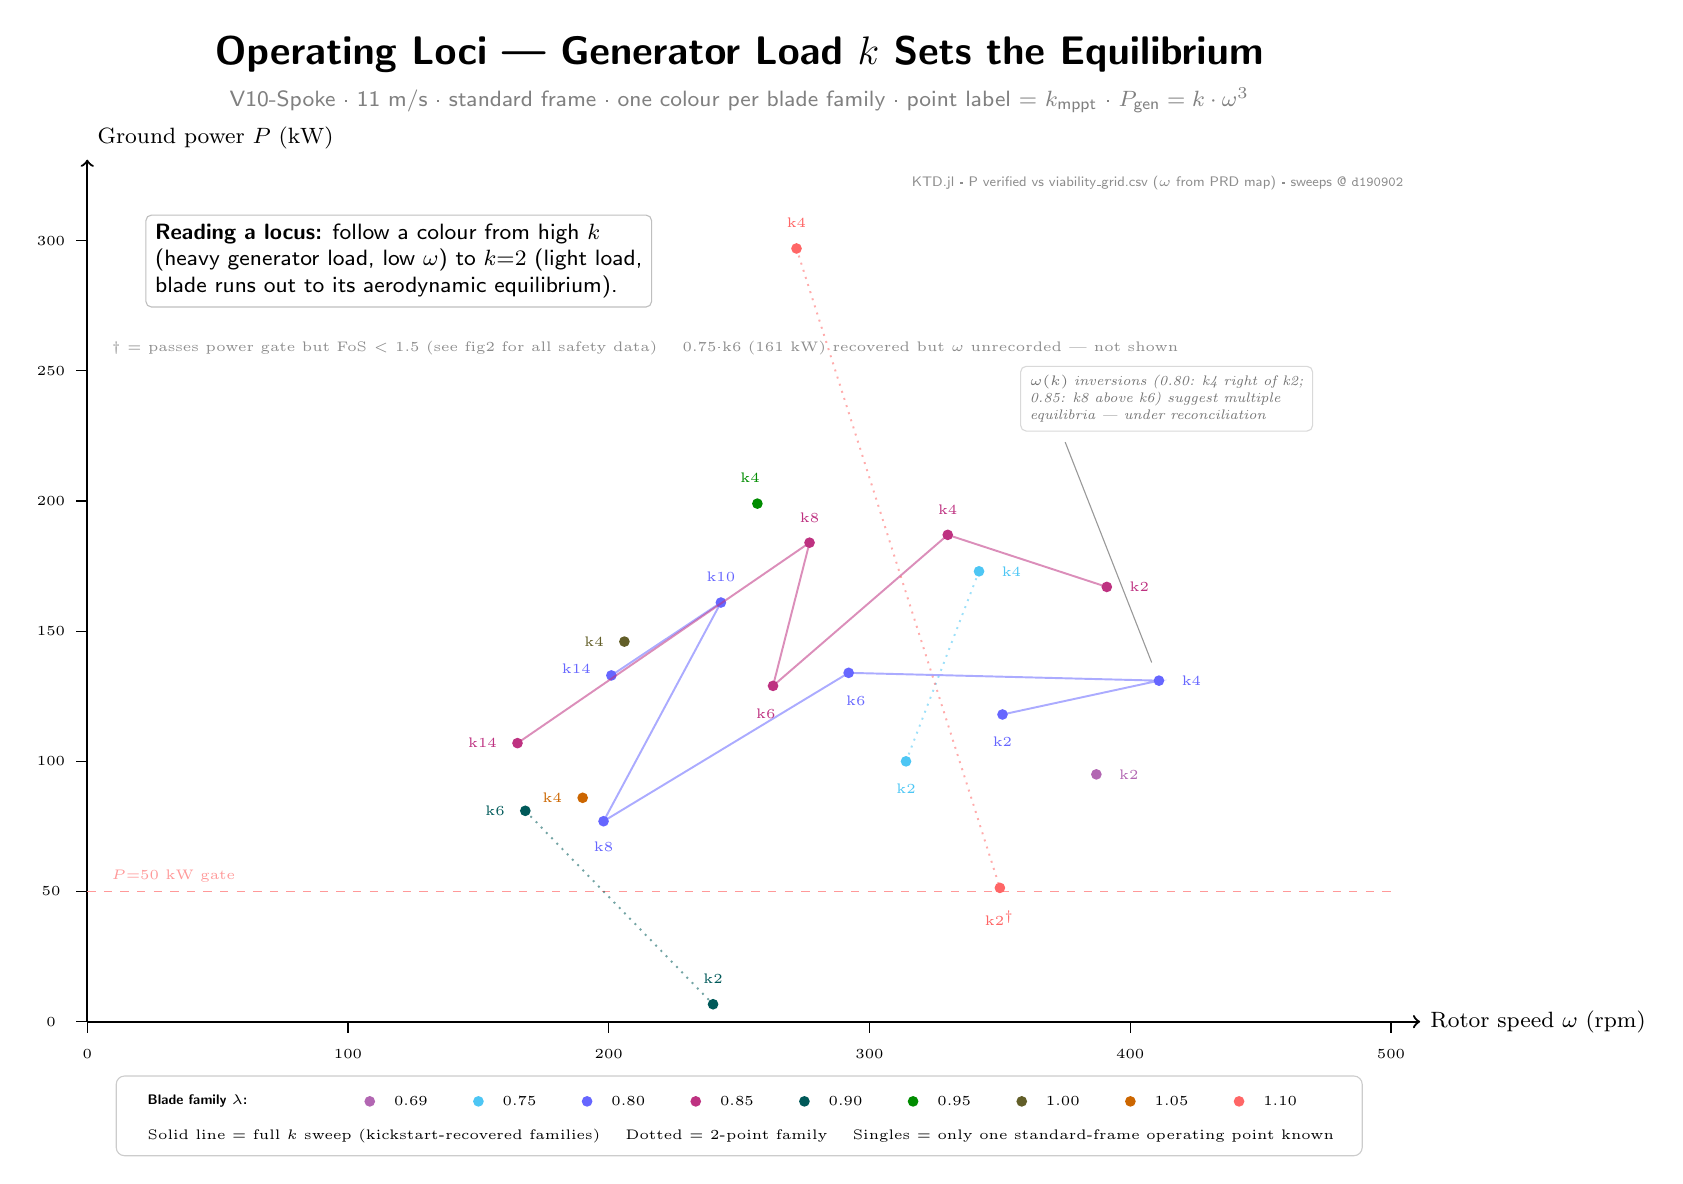
\begin{tikzpicture}[scale=0.92]

% fig4b (2026-07-16): second half of the retired fig4. One encoding: colour = blade
% family (same palette as fig2). Thin lines connect points of a family in k-order;
% each point is labelled with its k value. Standard frame only. No FoS (see fig2).
% Kickstart-swept families (0.69-0.85) have full k coverage; larger blades have
% catalog points only. Coordinate maps: x = 2.0 + omega*0.036, y = 2.0 + P*11.5/320

% ── Title ──
\node[font=\Large\sffamily\bfseries] at (11.0, 15.35) {Operating Loci — Generator Load $k$ Sets the Equilibrium};
\node[font=\footnotesize\sffamily, black!50] at (11.0, 14.72) {V10-Spoke · 11 m/s · standard frame · one colour per blade family · point label = $k_{\text{mppt}}$ · $P_{\text{gen}} = k\cdot\omega^3$};

% ── Axes ──
\draw[->, thick] (2.0, 2.0) -- (20.4, 2.0) node[right, font=\footnotesize] {Rotor speed $\omega$ (rpm)};
\draw[->, thick] (2.0, 2.0) -- (2.0, 13.9) node[above right, font=\footnotesize] {Ground power $P$ (kW)};
\foreach \w in {0,100,200,300,400,500} {
  \pgfmathsetmacro{\x}{2.0 + \w*0.036}
  \draw (\x, 1.85) -- (\x, 2.0);
  \node[font=\tiny] at (\x, 1.55) {\w};
}
\foreach \p in {0,50,100,150,200,250,300} {
  \pgfmathsetmacro{\y}{2.0 + \p*11.5/320}
  \draw (1.85, \y) -- (2.0, \y);
  \node[font=\tiny] at (1.5, \y) {\p};
}
\pgfmathsetmacro{\pg}{2.0 + 50*11.5/320}
\draw[dashed, red!40] (2.0, \pg) -- (20.0, \pg);
\node[font=\tiny, red!40, anchor=west] at (2.2, {\pg+0.22}) {$P{=}50$ kW gate};

% ── Family colours (consistent with fig2 legend, extended down to 0.69) ──
% 0.80-1.10 match fig2's palette; kickstart-only families (0.69, 0.75, 0.85) get
% their own hues — 0.85 deliberately magenta to echo fig4a's kickstart colour.
\colorlet{fam069}{violet!60}
\colorlet{fam075}{cyan!70}
\colorlet{fam080}{blue!60}
\colorlet{fam085}{magenta!75!black}
\colorlet{fam090}{teal!70!black}
\colorlet{fam095}{green!55!black}
\colorlet{fam100}{olive!60!black}
\colorlet{fam105}{orange!80!black}
\colorlet{fam110}{red!60}

% Helper: point + k label. \kpt{omega}{P}{colour}{k-label}{anchor}{dx}{dy}
\def\kpt#1#2#3#4#5#6#7{
  \fill[#3] ({2.0+#1*0.036}, {2.0+#2*11.5/320}) circle (2.1pt);
  \node[font=\tiny, #3, anchor=#5] at ({2.0+#1*0.036+#6}, {2.0+#2*11.5/320+#7}) {#4};
}

% ── λ=0.80 locus (kickstart sweep, k=2..14) — ordered k14→k2 ──
\draw[fam080, line width=0.7pt, opacity=0.55]
  ({2.0+201*0.036},{2.0+133*11.5/320}) -- ({2.0+243*0.036},{2.0+161*11.5/320}) --
  ({2.0+198*0.036},{2.0+77*11.5/320})  -- ({2.0+292*0.036},{2.0+134*11.5/320}) --
  ({2.0+411*0.036},{2.0+131*11.5/320}) -- ({2.0+351*0.036},{2.0+118*11.5/320});
\kpt{201}{133}{fam080}{k14}{east}{-0.15}{0.1}
\kpt{243}{161}{fam080}{k10}{south}{0}{0.15}
\kpt{198}{77}{fam080}{k8}{north}{0}{-0.15}
\kpt{292}{134}{fam080}{k6}{north}{0.1}{-0.18}
\kpt{411}{131}{fam080}{k4}{west}{0.18}{0}
\kpt{351}{118}{fam080}{k2}{north}{0}{-0.18}

% ── λ=0.85 locus (kickstart sweep, k=2..14) ──
\draw[fam085, line width=0.7pt, opacity=0.55]
  ({2.0+165*0.036},{2.0+107*11.5/320}) -- ({2.0+277*0.036},{2.0+184*11.5/320}) --
  ({2.0+263*0.036},{2.0+129*11.5/320}) -- ({2.0+330*0.036},{2.0+187*11.5/320}) --
  ({2.0+391*0.036},{2.0+167*11.5/320});
\kpt{165}{107}{fam085}{k14}{east}{-0.15}{0}
\kpt{277}{184}{fam085}{k8}{south}{0}{0.15}
\kpt{263}{129}{fam085}{k6}{north}{-0.1}{-0.18}
\kpt{330}{187}{fam085}{k4}{south}{0}{0.15}
\kpt{391}{167}{fam085}{k2}{west}{0.18}{0}

% ── λ=0.75 (kickstart, 2 pts) ──
\draw[fam075, line width=0.7pt, opacity=0.55, dotted]
  ({2.0+342*0.036},{2.0+173*11.5/320}) -- ({2.0+314*0.036},{2.0+100*11.5/320});
\kpt{342}{173}{fam075}{k4}{west}{0.18}{0}
\kpt{314}{100}{fam075}{k2}{north}{0}{-0.18}

% ── λ=0.69 (kickstart, 1 pt) ──
\kpt{387}{95}{fam069}{k2}{west}{0.18}{0}

% ── λ=0.90 (catalog, 2 pts: k6 viable, k2 rotating but underpowered) ──
\draw[fam090, line width=0.7pt, opacity=0.55, dotted]
  ({2.0+168*0.036},{2.0+81*11.5/320}) -- ({2.0+240*0.036},{2.0+6.7*11.5/320});
\kpt{168}{81}{fam090}{k6}{east}{-0.15}{0}
\kpt{240}{6.7}{fam090}{k2}{south}{0}{0.15}

% ── λ=0.95 (catalog, 1 pt) ──
\kpt{257}{199}{fam095}{k4}{south}{-0.1}{0.15}

% ── λ=1.00 (catalog, 1 pt) ──
\kpt{206}{146}{fam100}{k4}{east}{-0.15}{0}

% ── λ=1.05 (catalog, 1 pt) ──
\kpt{190}{86}{fam105}{k4}{east}{-0.15}{0}

% ── λ=1.10 (catalog, 2 pts: k4 viable, k2 fails FoS gate) ──
\draw[fam110, line width=0.7pt, opacity=0.55, dotted]
  ({2.0+272*0.036},{2.0+297*11.5/320}) -- ({2.0+350*0.036},{2.0+51.4*11.5/320});
\kpt{272}{297}{fam110}{k4}{south}{0}{0.15}
\kpt{350}{51.4}{fam110}{k2$^{\dagger}$}{north}{0}{-0.18}

% ── Annotations ──
\node[font=\footnotesize\sffamily, align=left, draw=black!25, rounded corners=2pt, fill=white] at (6.3, 12.5)
  {\textbf{Reading a locus:} follow a colour from high $k$\\
   (heavy generator load, low $\omega$) to $k{=}2$ (light load,\\
   blade runs out to its aerodynamic equilibrium).};

\node[font=\tiny\itshape, black!55, align=left, draw=black!15, rounded corners=2pt, fill=white] at (16.9, 10.6)
  {$\omega(k)$ inversions (0.80: k4 right of k2;\\
   0.85: k8 above k6) suggest multiple\\
   equilibria — under reconciliation};
\draw[black!40, thin] (15.5, 10.0) -- ({2.0+411*0.036-0.1}, {2.0+131*11.5/320+0.25});

\node[font=\tiny, black!45, anchor=west] at (2.2, 11.3)
  {$\dagger$ = passes power gate but FoS $<$ 1.5 (see fig2 for all safety data) \quad
   0.75·k6 (161 kW) recovered but $\omega$ unrecorded — not shown};

% ── Legend ──
\draw[rounded corners=3pt, fill=white, draw=gray!40] (2.4, 0.15) rectangle (19.6, 1.25);
\node[font=\tiny\sffamily\bfseries, anchor=west] at (2.7, 0.9) {Blade family $\lambda$:};
\foreach \l/\c/\xo in {0.69/fam069/0, 0.75/fam075/1.5, 0.80/fam080/3.0, 0.85/fam085/4.5, 0.90/fam090/6.0, 0.95/fam095/7.5, 1.00/fam100/9.0, 1.05/fam105/10.5, 1.10/fam110/12.0} {
  \fill[\c] (5.9+\xo, 0.9) circle (2.1pt);
  \node[font=\tiny, anchor=west] at (6.1+\xo, 0.9) {\l};
}
\node[font=\tiny, anchor=west] at (2.7, 0.42)
  {Solid line = full $k$ sweep (kickstart-recovered families) \quad Dotted = 2-point family \quad
   Singles = only one standard-frame operating point known};

% ── Provenance ──
\node[font=\tiny\sffamily, black!45, anchor=south east] at (20.3, 13.35)
  {KTD.jl · P verified vs viability\_grid.csv ($\omega$ from PRD map) · sweeps @ \texttt{d190902}};

\end{tikzpicture}
\end{document}
